\section{results}
Here, results, in the form of the visual methods described in the previous section, are presented. 
Only descriptions of the plots, and why certain values were picked is discussed here. 
For thorough discussion and analysis of the results, see the section for discussion and analysis.
In order to make results somewhat comparable, an attempt to keep the parameters the same as much as possible is made.

\subsection{Error and accuracy}
The first results presented are some statistics for the simplest case with only $a$, $b$ and $c$ considered.

\begin{figure}[H]
    \centering
    \subfloat[]{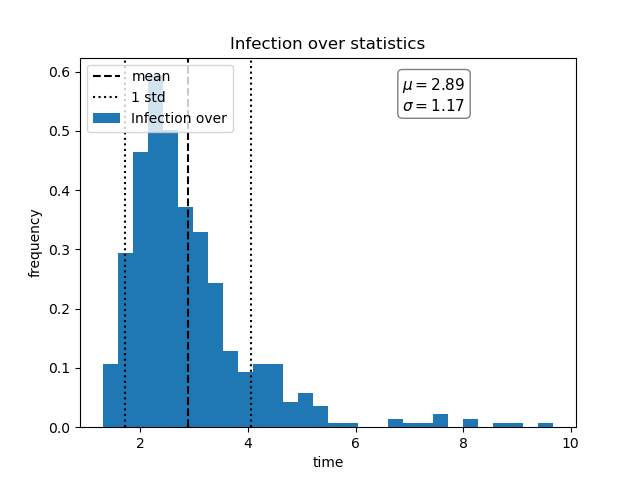
\includegraphics[scale=0.55]{plots/MC_solver_multiple_a_4_b_4_c_0.5500over_I500.png}}
    \subfloat[]{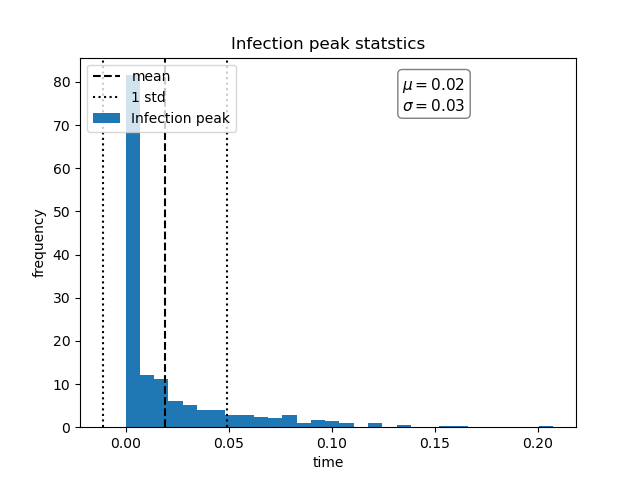
\includegraphics[scale=0.55]{plots/MC_solver_multiple_a_4_b_4_c_0.5500Peak_I500.png}}
    \caption{The time taken for the when the infection is over (a), and when the ifection peaks (b) $a=4$, $b=4$ and $c=0.5$ run 500 times each}
    \label{fig:error_IoverIpeak}
\end{figure}

In \textit{Figure} \ref{fig:error_IoverIpeak}, a simulation is ran with $a=4$, $b=4$ and $c=0.5$ 500 times, where we expect an initial peak of infections, before the infection dies out completely.

In \textit{Figure} \ref{fig:error_meanI}, the mean value of the number of infections after reaching a steady state is calculated.

\begin{figure}[H]
    \centering
    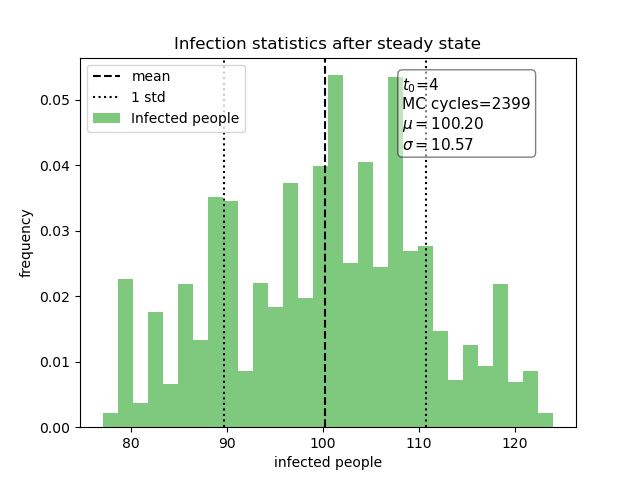
\includegraphics[scale=0.55]{plots/MC_solver_error_a_4_b_1_c_0.5I_SS_mcs_2399.png}
    \caption{MC statistics after the steady state with $a=4$, $b=1$ and $c=0.5$ for 500 runs}
    \label{fig:error_meanI}
\end{figure}

\subsection{Changing $b$}
The first scenario to be considered, is with only $a$, $b$ and $c$.
To keep things simple, only b will change such that $b\in \{1,2,3,4\}$.
\begin{figure}[H]
    \centering
    \subfloat[]{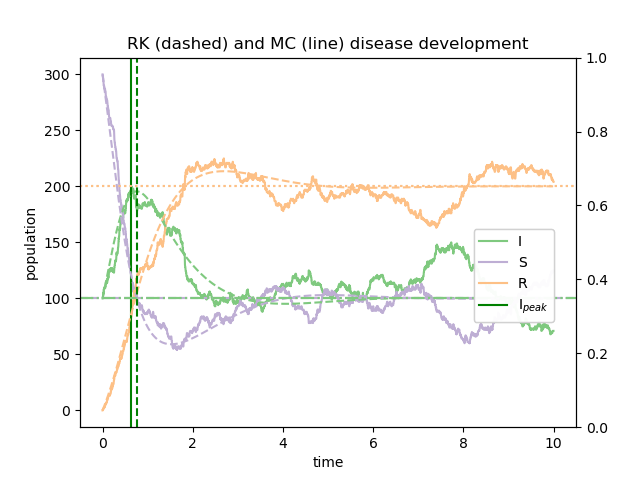
\includegraphics[scale=0.5]{plots/Compare_bbb_a_4_b_1_c_0.5.png}}
    \subfloat[]{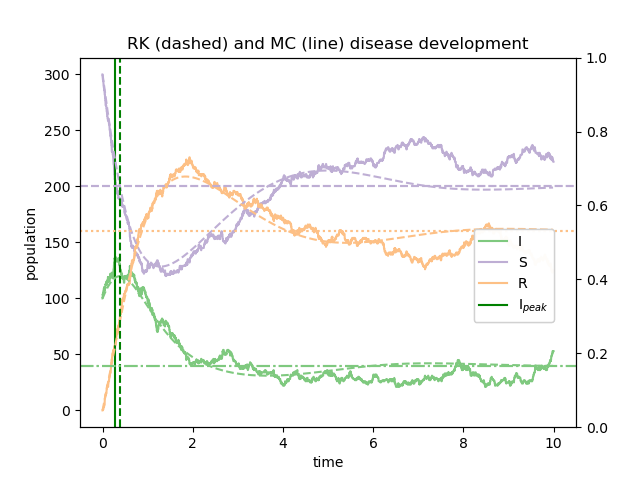
\includegraphics[scale=0.5]{plots/Compare_bbb_a_4_b_2_c_0.5.png}}\\
    \subfloat[]{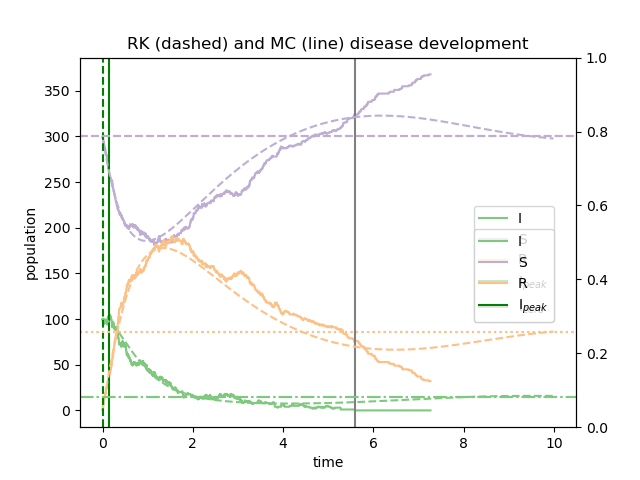
\includegraphics[scale=0.5]{plots/Compare_bbb_a_4_b_3_c_0.5.png}}
    \subfloat[]{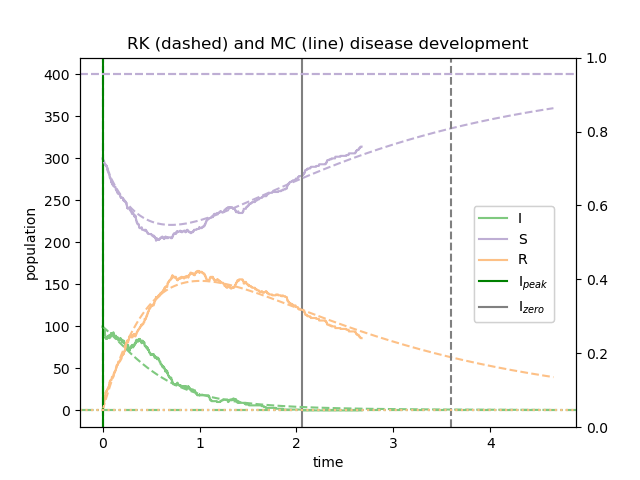
\includegraphics[scale=0.5]{plots/Compare_bbb_a_4_b_4_c_0.5.png}}
    \caption{Comparison of RK solver (dashed) and MC simulation (line) with expected values (horizontal dashed) with fixed $a=4$ and $c=0.5$. 
    $b$ has values 1(a), 2(b), 3(c) and 4(d). The horizontal dashed lines are the expected values.}
    \label{fig:b}
\end{figure}
In \textit{Figure} \ref{fig:b}, the RK and MC approach the expected values, and we see that the infection manages to reach steady state within the population for $b=1$ and $b=2$.

\subsection{Vital Parameters}
The next scenatio to be considered is including vital parameters narutal death $d$, natural birth $e$ and death due to disease $d_I$.
Having a ridiculously high birth rate or natural death rate doesn't really make any sense here, as it would either kill everyone or explode the population.
Ideally we want the population to be somewhat stable, and see how disease deaths influence the steady state of the system.
The key aspect here, is that when people die from the infection, it keeps them from infecting others, essentially killing the disease by removing carriers of the disease.
To explore this further, $e=0.011$ and $d=0.01$, while $d_I$ varies. 
Having the birthrate slightly higher than the natural death rate, makes the infection deaths decide whether the population is increasing or decreasing, which makes interpretation of the plots easier.
Some key plots will be included to show how $d_I$ affects the steady state, and how fast the infection is over.


\begin{figure}[H]
    \centering
    \subfloat[]{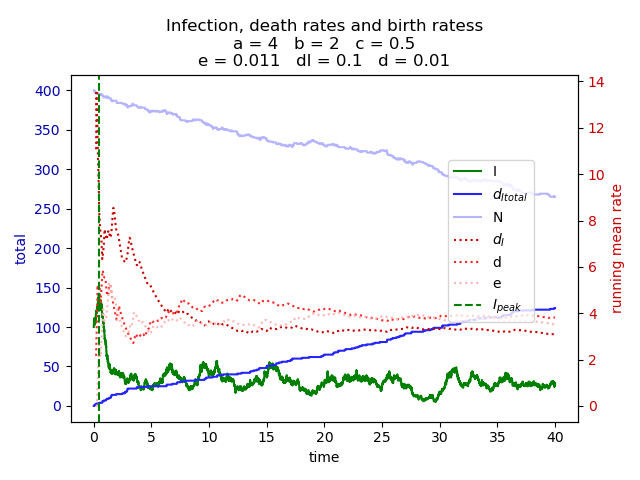
\includegraphics[scale=0.5]{plots/MC_solver_vital_a_4_b_2_c_0.5_IdI0.1.png}}
    \subfloat[]{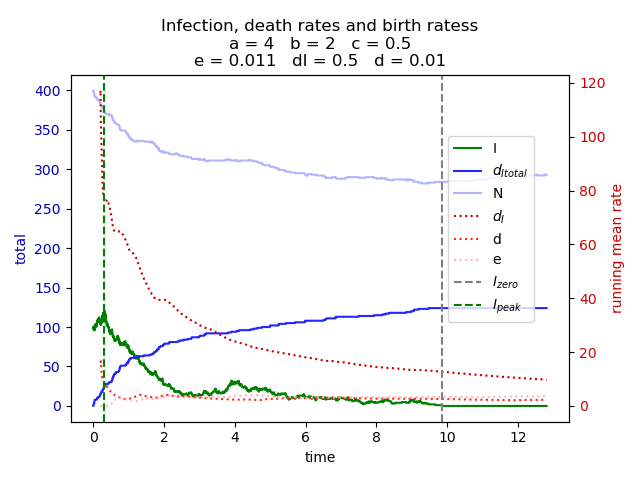
\includegraphics[scale=0.5]{plots/MC_solver_vital_a_4_b_2_c_0.5_IdI0.5.png}}\\
    \subfloat[]{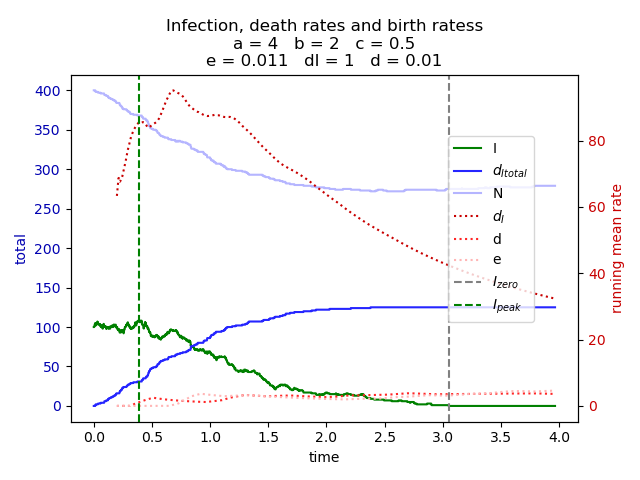
\includegraphics[scale=0.5]{plots/MC_solver_vital_a_4_b_2_c_0.5_IdI1.png}}
    \subfloat[]{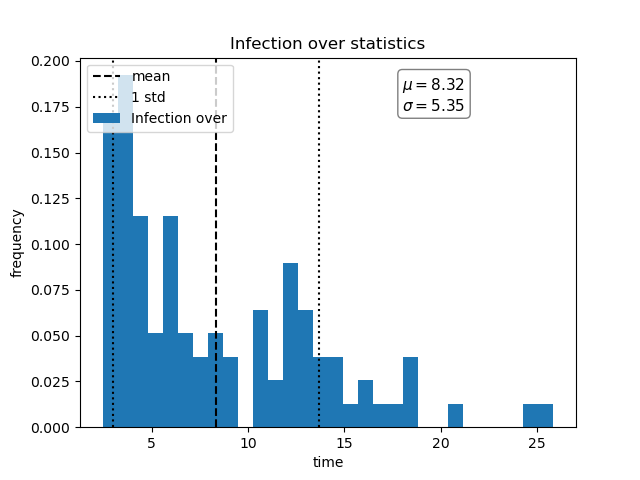
\includegraphics[scale=0.5]{plots/MC_solver_multiple_a_4_b_2_c_0.5100over_I100dI1.png}}
    \caption{Disease development for $a=4$, $b=2$, $c=0.5$, $e=0.011$ and $d=0.01$. $d_I$ varies as 0.1 (a), 0.5(b) and 1(c and d), with 100 runs collecting the statistics in (d)}
    \label{fig:vitalb2}
\end{figure}

In \textit{Figure} \ref{fig:vitalb2}, varying values of $d_I$ are shown for the previously stable case where $b=2$. 


In the case of the MC solver, having $d_I$ high may cause the disease to die faster due to randomness. To test this further, a smaller amount of initial infections are tested, to see if a high death rate actually prevents a disease to spread.
In \textit{Figure} \ref{fig:vitalI20} the initial infections are set to 20, but the disease development is still the same, just with a lower peak than before. 
Here, it is hard to tell whether the total deaths are lower or higher, since when we start with 100 indected, leading up getting 100 infected, a lot of people probably died.
So, the most reasonable thing to look at is the height of the infection peak, and the death rate, which is lower in the case with initial $I=20$, meaning that a higher deathrate probably reduces the infection peak deaths by killing carriers.
\begin{figure}[H]
    \centering
    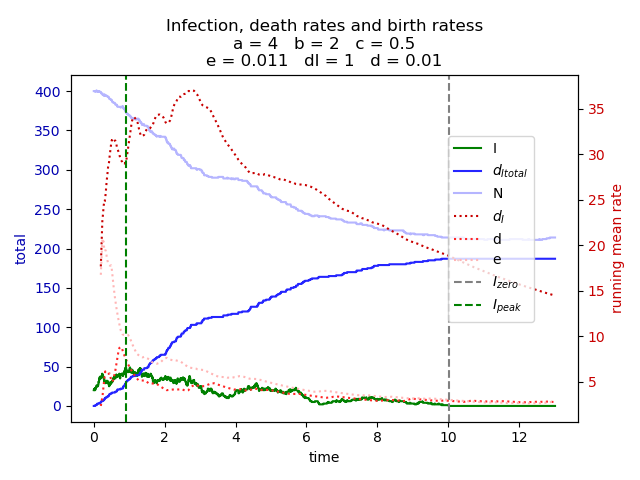
\includegraphics[scale=0.55]{plots/MC_solver_vitalI20_a_4_b_2_c_0.5_IdI1.png}
    \caption{A run with initial infections = 20, with $a=4$, $b=2$, $c=0.5$, $e=0.011$, $d=0.01$ and $d_I=1$.}
    \label{fig:vitalI20}
\end{figure}


\subsection{Seasonal Variation}
Another parameter that impacts things like the flu in particular, is seasonal variations.
To simulate this, the rate of infection $a_{seasonal}$ is modyfied by
$$
a_{seasonal}=a+Acos(\omega t)
$$
To explore this, $\omega = 2 \pi$, and $A \in \{1,2,3,4\}$ for $a=4$, $b=2$ or $b=1$ and $c=0.5$. Initially, no vital parameters will be introduced.

\begin{figure}[H]
    \centering
    \subfloat[]{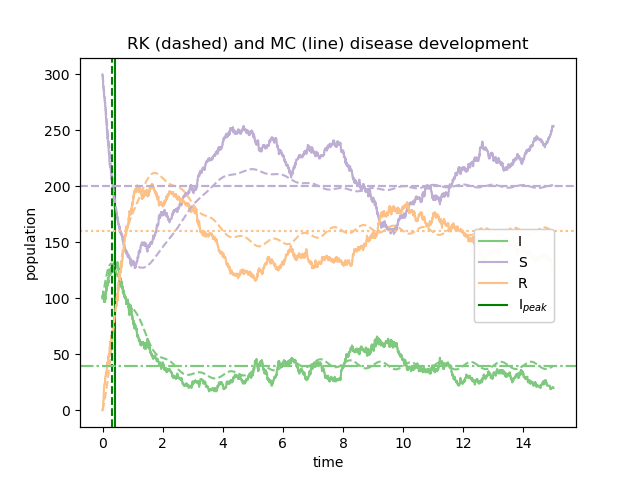
\includegraphics[scale=0.5]{plots/Compare_seasonalA1_a_4_b_2_c_0.5.png}}
    \subfloat[]{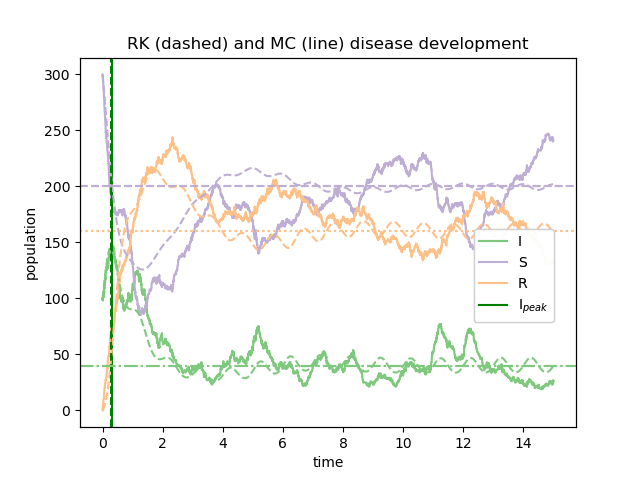
\includegraphics[scale=0.5]{plots/Compare_seasonalA2_a_4_b_2_c_0.5.png}}\\
    \subfloat[]{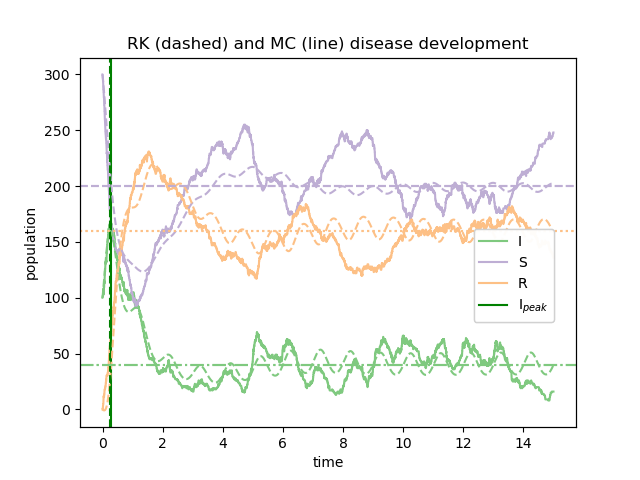
\includegraphics[scale=0.5]{plots/Compare_seasonalA3_a_4_b_2_c_0.5.png}}
    \subfloat[]{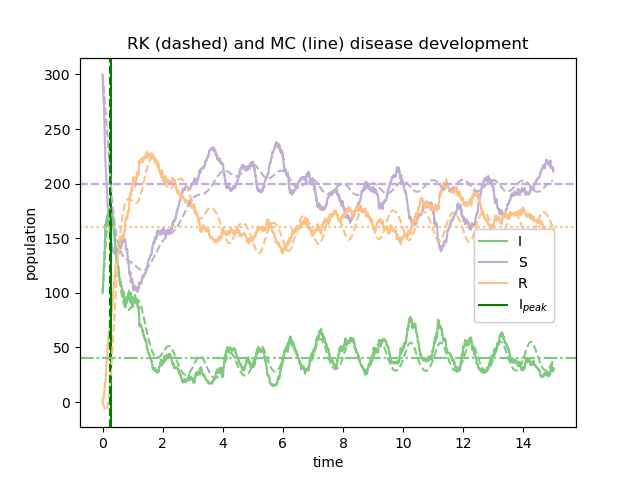
\includegraphics[scale=0.5]{plots/Compare_seasonalA4_a_4_b_2_c_0.5.png}}
    \caption{Disease development for $a=4$, $b=2$, $c=0.5$, with seasonal variation amplitude $A \in \{1,2,3,4\}$.}
    \label{fig:seasonalb2}
\end{figure}

Changing $b$ so that $b=1$ causes the expected values for $I$ and $S$ to be the same, highlighting the cyclic relationship of the two, as seen in In \textit{Figure} \ref{fig:seasonalb1}

\begin{figure}[H]
    \centering
    \subfloat[]{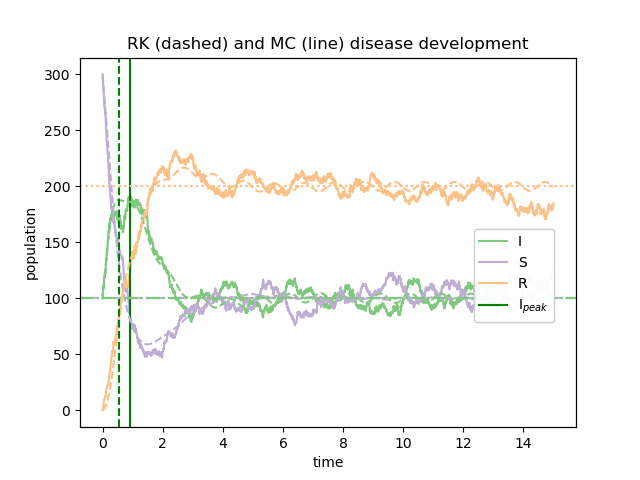
\includegraphics[scale=0.5]{plots/Compare_seasonalA1_a_4_b_1_c_0.5.png}}
    \subfloat[]{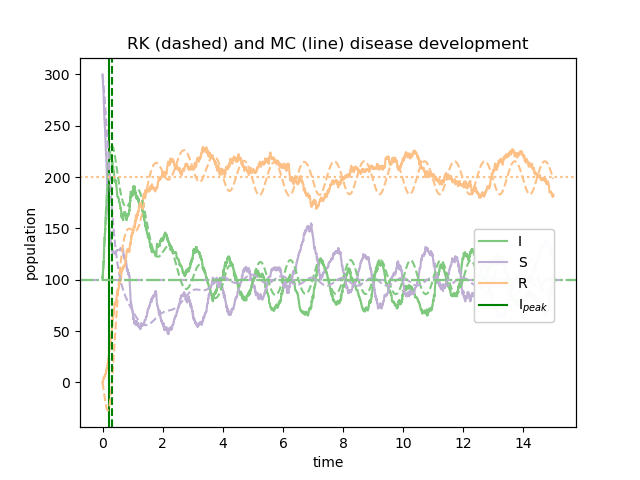
\includegraphics[scale=0.5]{plots/Compare_seasonalA4_a_4_b_1_c_0.5.png}}
    \caption{Disease development for $a=4$, $b=1$, $c=0.5$, with seasonal variation amplitude $A \in \{1,4\}$.}
    \label{fig:seasonalb1}
\end{figure}

So how does this affect the statistics of when an infection is over, or the mean amount of infected people? 
In \textit{Figure} \ref{fig:seasonal_SS} the mean remains the same as in \textit{Figure} \ref{fig:error_meanI}, but $\sigma$ is higher.

\begin{figure}[H]
    \centering
    \subfloat[]{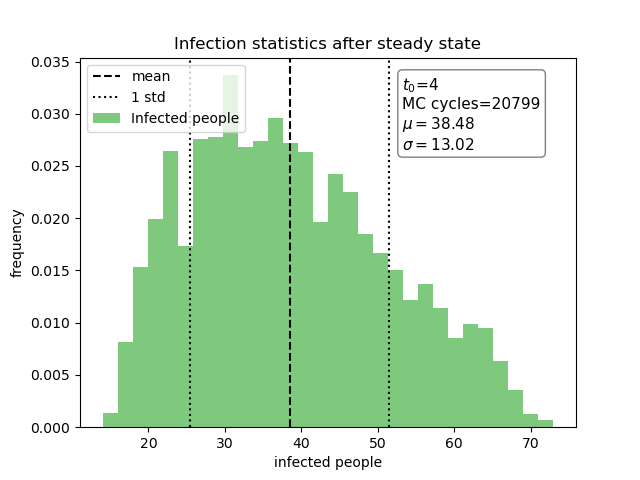
\includegraphics[scale=0.5]{plots/MC_solver_seasonalA4_a_4_b_2_c_0.5I_SS_mcs_2079920798.png}}
    \subfloat[]{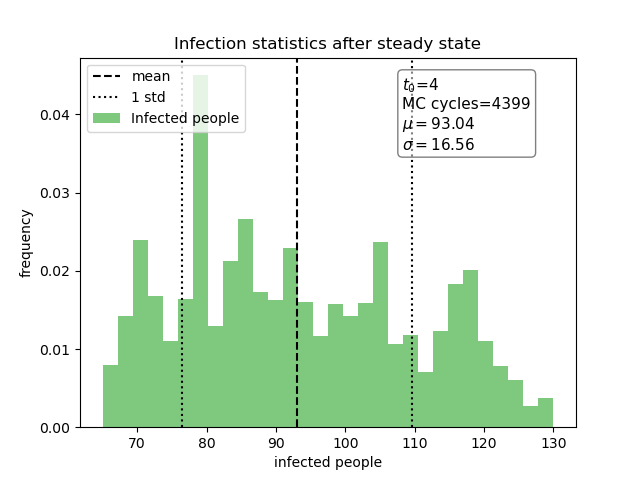
\includegraphics[scale=0.5]{plots/MC_solver_seasonalA4_a_4_b_1_c_0.5I_SS_mcs_43994398.png}}
    \caption{Disease statistics for Infections after steady state for $a=4$, $b=1$ (a) and $b=2$ (b), $c=0.5$, with seasonal variation amplitude $A = 4$.}
    \label{fig:seasonal_SS}
\end{figure}



\begin{figure}[H]
    \centering
    \subfloat[]{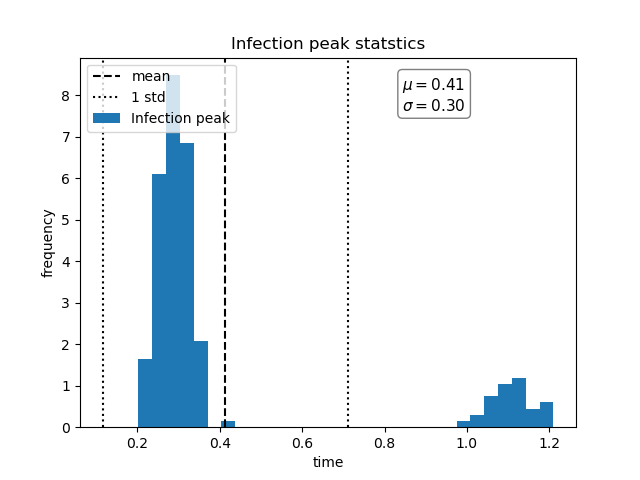
\includegraphics[scale=0.5]{plots/MC_solver_multiple_a_4_b_1_c_0.5200Peak_I200.png}}
    \subfloat[]{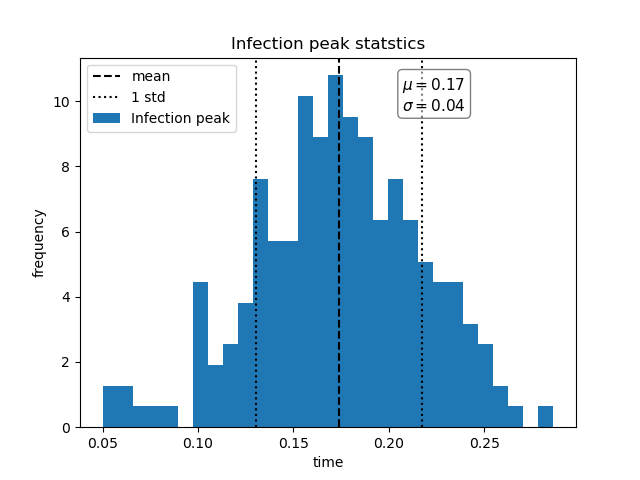
\includegraphics[scale=0.5]{plots/MC_solver_multiple_a_4_b_2_c_0.5200Peak_I200.png}}
    \caption{Infection peak for $a=4$, $b=1$ (a) and $b=2$ (b), $c=0.5$, with seasonal variation amplitude $A = 4$, and vital parameters $e=0.011$, $d=0.01$ and $d_I=1$ collecting statistics over 200 runs.}
    \label{fig:seasonalI_peak}
\end{figure}s
In \textit{Figure} \ref{fig:seasonalI_peak} (a), there is actually a chance of having a delayed peak on the second cycle, rather than the first.
This however is not the case in (b). In \textit{Figure} \ref{fig:seasonalI_peak}, compared to \textit{Figure} \ref{fig:vitalb2}, the $\sigma$ values are about the same, so no here the seasonal variation's effect is inconclusive.

\begin{figure}[H]
    \centering
    \subfloat[]{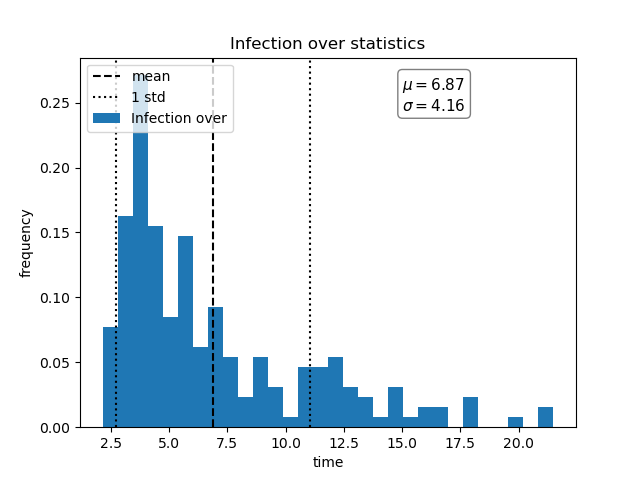
\includegraphics[scale=0.5]{plots/MC_solver_multiple_a_4_b_2_c_0.5200over_I200.png}}
    \caption{Infection over for $a=4$, $b=2$, $c=0.5$, with seasonal variation amplitude $A = 4$, and vital parameters $e=0.011$, $d=0.01$ and $d_I=1$ collecting statistics over 200 runs.}
    \label{fig:seasonalI_over}
\end{figure}



\subsection{Vaccines}
The next scenario to be considered is vaccines. The case studied here in particular, is how vaccines can prevent deaths, and flatten and reduce the peak of the infection curve.
In \textit{Figure} \ref{fig:latevacc}, the simulation is stared at $I=100$, meaning that many already are infected, so here vaccination will cause the amount of infected people do drop faster, due to fewer being susceptible.
Is the inital conditions are close to the peak, the actual peak is mostly unaffected, with the disease duration being the main thing that is changed.
However, in (b) and (d), the total deaths are much lower in (d), with a similar amount of total vaccines given. Thus, vaccinating many fast is better than many slow.
\begin{figure}[H]
    \centering
    \subfloat[]{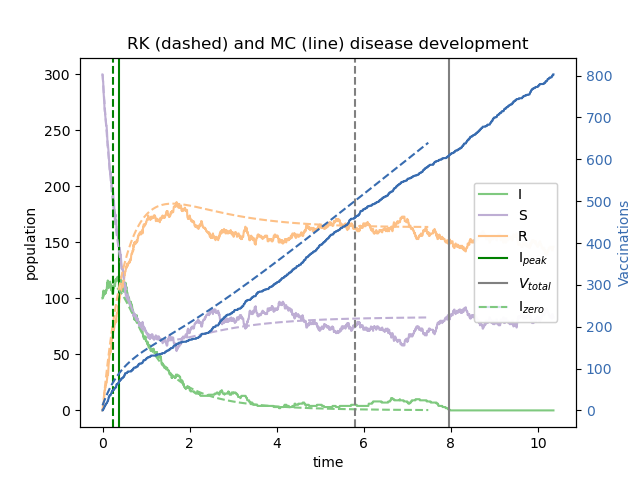
\includegraphics[scale=0.5]{plots/Compare_vaccines_a_4_b_1_c_0.5_f_1.png}}
    \subfloat[]{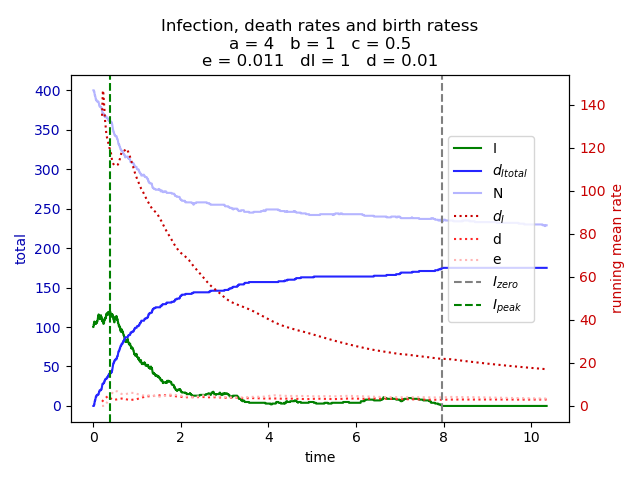
\includegraphics[scale=0.5]{plots/MC_solver_vaccines_a_4_b_1_c_0.5_f_1_IdI.png}}\\
    \subfloat[]{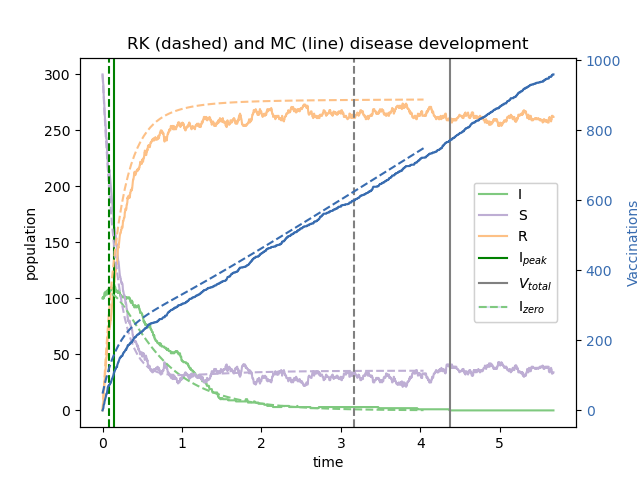
\includegraphics[scale=0.5]{plots/Compare_vaccines_a_4_b_1_c_0.5_f_4.png}}
    \subfloat[]{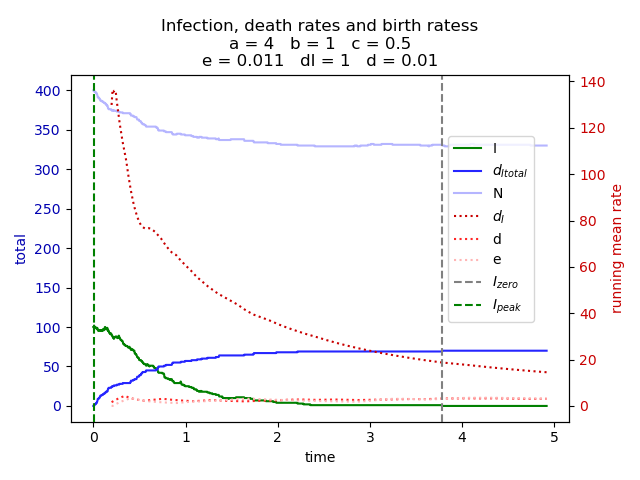
\includegraphics[scale=0.5]{plots/MC_solver_vaccines_a_4_b_1_c_0.5_f_8_IdI.png}}
    \caption{Disease development for $a=4$, $b=1$, $c=0.5$, with vaccination rates $f=1$ (a and b) and $f=8$ (c and d)}
    \label{fig:latevacc}
\end{figure}

In \textit{Figure} \ref{fig:earlyvacc}, vaccines are introduced early, starting the simulation at $I=20$. 
From \textit{Figure} \ref{fig:vitalI20}, we saw that starting the simulate early at $I=20$, produces the same kind of peak than starting later, given that there are no factors such as very high disease death rate significantly halting the disease on its way to its pieak.
Vaccination can be considered one suck peak reducing factor, as seen in In \textit{Figure} \ref{fig:earlyvacc}, where early vaccination of just $f=0.5$ drastically reduces total deaths.
For $f=1$ and $f=2$ in (c) and (d), this effect is even more dramatic. So, introducing vaccines early can have a very severe impact on the total deaths due to the disease.
\begin{figure}[H]
    \centering
    \subfloat[]{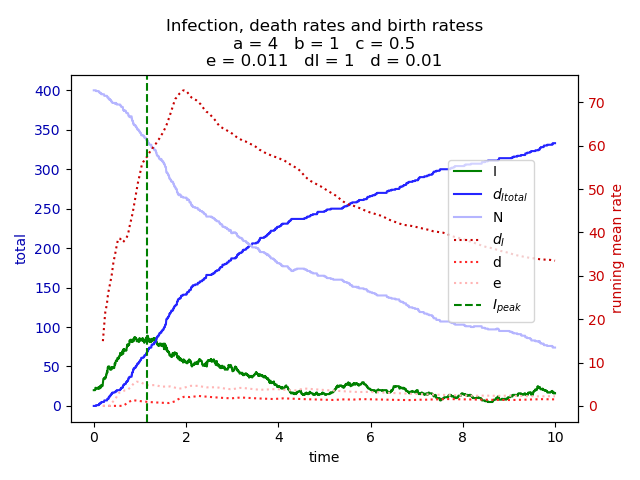
\includegraphics[scale=0.5]{plots/MC_solver_vaccinesI20_a_4_b_1_c_0.5_IdI.png}}
    \subfloat[]{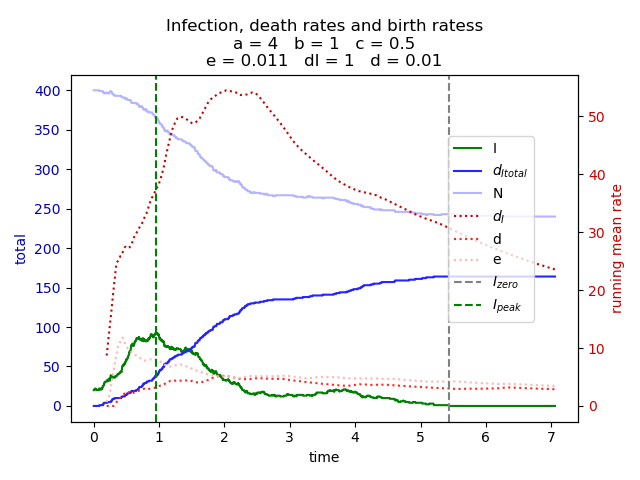
\includegraphics[scale=0.5]{plots/MC_solver_vaccinesI20_a_4_b_1_c_0.5_f_0.5_IdI.png}}\\
    \subfloat[]{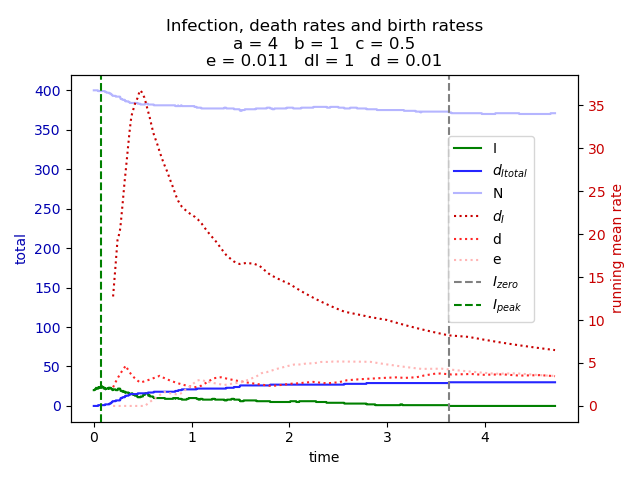
\includegraphics[scale=0.5]{plots/MC_solver_vaccinesI20_a_4_b_1_c_0.5_f_1_IdI.png}}  
    \subfloat[]{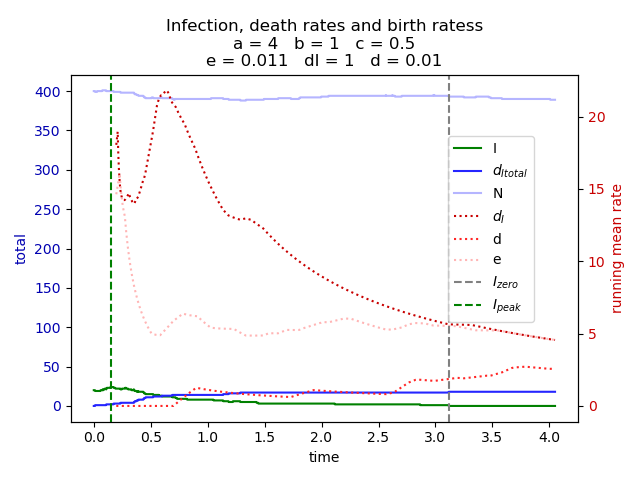
\includegraphics[scale=0.5]{plots/MC_solver_vaccinesI20_a_4_b_1_c_0.5_f_4_IdI.png}}
    \caption{Vaccination rates effect on disease development for $a=4$, $b=1$, $c=0.5$, with vaccination rates $f=0$ (a), $f=0.5$ (b), $f=1$ (c), $f=4$ (d)}
    \label{fig:earlyvacc}
\end{figure}
